\documentclass[a4paper,10pt,twoside]{article}
%\usepackage{amssymb}
%\usepackage{amsthm}
\usepackage[polish]{babel}
\usepackage[utf8]{inputenc}
\usepackage[T1]{fontenc}
\usepackage{indentfirst}
\usepackage[top=2.5cm, bottom=2.5cm, left=2.5cm, right=2.5cm]{geometry}
\usepackage{graphicx}
\usepackage{amsmath}

\begin{document}

\begin{center}
\bgroup
\def\arraystretch{1.5}
\begin{tabular}{|c|c|c|c|c|c|}
	\hline
	EAIiIB & \multicolumn{2}{|c|}{\begin{tabular}{@{}c@{}}Marcin Nalepa \\ Przemysław Trybała\end{tabular}} & Rok II & Grupa 5 & Zespół 3 \\
	\hline
	\multicolumn{3}{|c|}{\begin{tabular}{c}Temat: \\ Współczynnik załamania światła dla ciał stałych \end{tabular}} & 
	\multicolumn{3}{|c|}{\begin{tabular}{c}Numer ćwiczenia: \\ 51 \end{tabular}} \\
	\hline
	\begin{tabular}{@{}c@{}}Data wykonania\\\phantom{data}\end{tabular} & \begin{tabular}{@{}c@{}}Data oddania\\\phantom{data}\end{tabular} & 
	\begin{tabular}{c}Zwrot do\\poprawki\\\phantom{data} \end{tabular} & \begin{tabular}{c}Data oddania\\\phantom{data}\end{tabular} &
	\begin{tabular}{@{}c@{}}Data zaliczenia\\\phantom{data}\end{tabular} & \begin{tabular}{c}Ocena\\\phantom{ocena}\end{tabular} \\[4ex]
	\hline
\end{tabular}
\egroup
\end{center}

\section{Cel ćwiczenia}
Celem ćwiczenia jest wyznaczenie współczynnika załamania światła dla szkła i
zbadanie jego zmian w zależności od długości fali światła padającego.

\section{Wstęp teoretyczny}
Światło padające na granicę dwóch ośrodków ulega dwóm zjawiskom, odbiciu i załamaniu.
Prawo załamania - stosunek sinusa kąta padania do sinusa kąta załamania jest równy stosunkowi bezwzględnego współczynnika
załamania ośrodka drugiego $n_2$ do bezwzględnego współczynnika załamania ośrodka pierwszego $n_1$, czyli współczynnikowi
względnemu załamania światła ośrodka drugiego względem pierwszego. Jest to tzw. prawo Snelliusa.

Współczynnik załamania zależy od długości fali światła padającego. Poprzez proste przekształcenia trygonometryczne, korzystając
z zależności $\lambda = VT$, otrzymujemy
\begin{equation}
\frac{\sin\alpha}{\sin\beta}=\frac{V_1}{V_2}=\frac{\lambda_1}{\lambda_2}=\frac{n_1}{n_2}=n=const
\end{equation}
gdzie $\alpha$ - kąt padania, $\beta$ - kąd załamanej wiązki światła, $n$ - współczynnik załamania światła ośrodka 2 względem 1.

Z tego względu załamanie może być wykorzystane do rozłożenia wiązki światła na składowe o różnych długościach fali co jest
widoczne na przykład w pryzmacie.
	
\section{Opis doświadczenia}
Do doświadczenia zostały użyte szklana płytka i mikroskop ze śrubą mikrometryczną. Na płytce zostały zaznaczone markerem linie
poziome i pionowe z różnych jej stron. Za pomocą śruby mikrometrycznej została zmierzona grubość płytki. Następnie płytkę
umieszczono pod mikroskopem. Wykorzystując małe pole ostrości mikroskopu i śrubę mikrometryczną mierzącą wysokość tacki można
odczytać grubość pozorną. Doświadczenia zostały powtórzone dla filtrów barwnych: czerwony(630nm), żółty(590nm),
zielony(500nm) i niebieski(480nm). Wyniki zapisano w tabelach.

\section{Wyniki pomiarów}
Dołączone tabele z wynikami.

\newpage
\section{Opracowanie wyników}

\begin{figure}[!htp]
\centerline{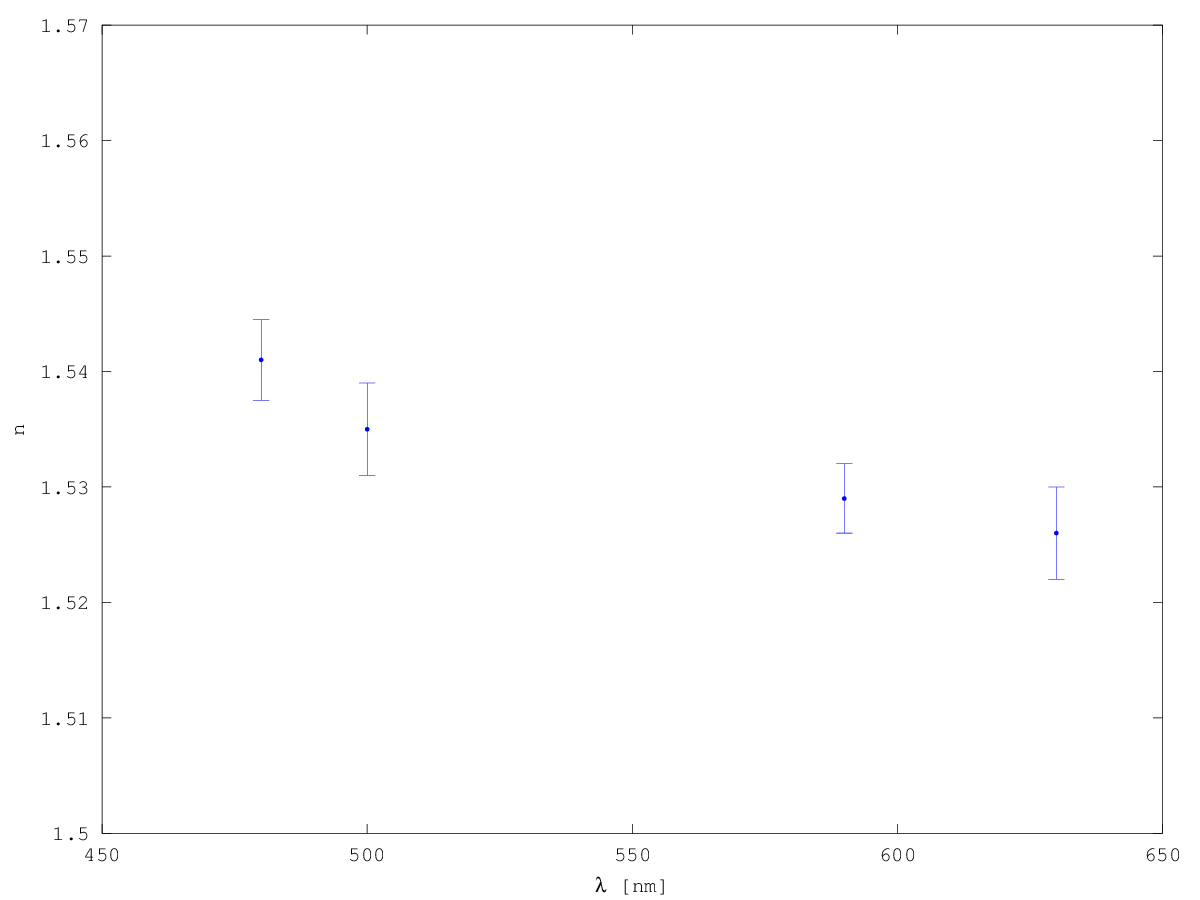
\includegraphics[scale=0.5]{image-disperse}}
\caption{Wykres zależnosci długości fali od współczynnika załamania}
\label{fig:nlambda}
\end{figure}

\begin{table}[!htp]
\def\arraystretch{1.4}
\centering
\begin{tabular}{|l|l|l|l|l|}
\hline
             & h     & u(h)  & n     & u(n)   \\ \hline
biały        & 3.152 & 0.007 & 1.537 & 0.0035 \\ \hline
czerwony     & 3.174 & 0.008 & 1.526 & 0.0040 \\ \hline
pomarańczowy & 3.169 & 0.006 & 1.529 & 0.0030 \\ \hline
zielony      & 3.156 & 0.008 & 1.535 & 0.0040 \\ \hline
niebieski    & 3.145 & 0.007 & 1.537 & 0.0035 \\ \hline
\end{tabular}
\end{table}
\noindent
Wzór na wartość współczynnika załamania $n=\frac{d}{h}$ gdzie $d$ - grubość rzeczywista, a $h$ grubość pozorna.
\noindent
Wzór na niepewność współczynnika załamania $n$
$$u(n)=n*\sqrt{\left(\frac{u(d)}{d} \right )^2 + \left(\frac{u(h)}{h} \right )^2}$$
Dla światła białego
$$u(n)=1.537*\sqrt{\left (\frac{0.003}{4.845} \right )^2 + \left (\frac{0.007}{3.152} \right )^2}=1.537*\sqrt{3.834\times {10}^-7 + 4.932\times {10}^-6}=1.537*0.0023=0.0035$$
Wyliczone wartości dla kolorowych szkiełek
\begin{equation}
\label{eq:wyniki}
\begin{split}
u_{niebieskie}(n)&=0.0035 \\
u_{zielone}(n)&=0.0040 \\
u_{pomaranczowe}(n)&=0.0030 \\
u_{czerwone}(n)&=0.0040 \\
\end{split}
\end{equation}
Wartości dla wszystkich kolorów zostały wpisane razem z niepewnościami z równań (\ref{eq:wyniki}) do tabelki,
a następnie posłużyły jako źródło do narysowania wykresu (\ref{fig:nlambda}).

\newpage
\section{Podsumowanie}
Na wykresie widać tendencję wyników do spadku wraz ze wzrostem długości fali, w szczególności wyniki dla światła
niebieskiego, a pomarańczowego i czerwonego nie pokrywają się nawet w granicach błędu.
Na tej podstawie można wysunąć wniosek że współczynnik załamania maleje wraz ze wzrostem długości fali światła.
Jednak na podstawie wyników nie można powiedzieć czy jest to oczekiwany spadek wykładniczy, ponieważ zakres badanych
długości fali jest zbyt ograniczony.


\end{document}


























